\chapter{Aerodynamic Characteristics}

\section{Aerodynamic Characteristics Approximation}

\subsection{Lift Coefficient Approximation}

\begin{figure}[h!]
  \centering
  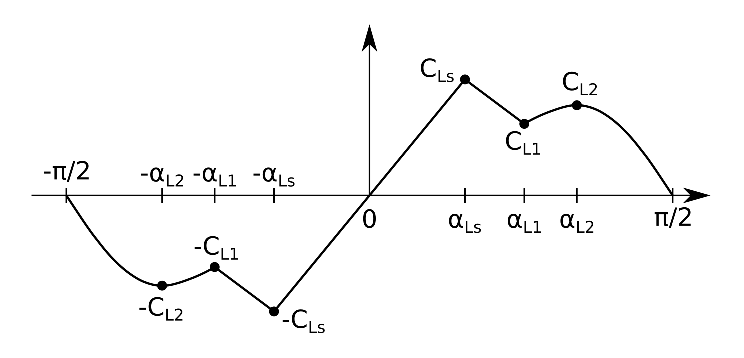
\includegraphics[width=120mm]{eps/approx_cz.eps}
  \caption{Lift coefficient approximation}
\end{figure}

Following approximation is used to get lift coefficient for the full range of angle of attack. \cite{NASA-TM-102267}

Lift coefficient is given by the following expressions:
\begin{multline}
  C_L =
  -
  \frac{
    \left( \alpha + \alpha_{L2} \right)
    \left( \alpha + \frac{\pi}{2} \right) 
  }
  {
    \left( \alpha_{L1} - \alpha_{L2} \right)
    \left( \alpha_{L1} - \frac{\pi}{2} \right) 
  } C_{L1}
  -
  \frac{
    \left( \alpha + \alpha_{L1} \right)
    \left( \alpha + \frac{\pi}{2} \right)
  }
  {
    \left( \alpha_{L2} - \alpha_{L1} \right)
    \left( \alpha_{L2} - \frac{\pi}{2} \right)
  } C_{L2} \\
  \mathrm{~for~} -\frac{\pi}{2} \leq \alpha \leq - \alpha_{L1}
\end{multline}
\begin{align}
  C_L &=
  \frac{ C_{L1} - C_{Ls} }{ \alpha_{L1} - \alpha_{Ls} }
  \left( \alpha + \alpha_{Ls} \right) - C_{Ls}
  \mathrm{~for~} - \alpha_{L1} < \alpha \leq - \alpha_{Ls} \\
  C_L &= \frac{C_{Ls}}{\alpha_{Ls}} \alpha
  \mathrm{~for~} - \alpha_{Ls} < \alpha < \alpha_{Ls} \\
  C_L &=
  \frac{ C_{L1} - C_{Ls} }{ \alpha_{L1} - \alpha_{Ls} }
  \left( \alpha - \alpha_{Ls} \right) + C_{Ls}
  \mathrm{~for~} \alpha_{Ls} \leq \alpha < \alpha_{L1}
\end{align}
\begin{multline}
  C_L =
  \frac{
    \left( \alpha - \alpha_{L2} \right)
    \left( \alpha - \frac{\pi}{2} \right) 
  }
  {
    \left( \alpha_{L1} - \alpha_{L2} \right)
    \left( \alpha_{L1} - \frac{\pi}{2} \right) 
  } C_{L1}
  +
  \frac{
    \left( \alpha - \alpha_{L1} \right)
    \left( \alpha - \frac{\pi}{2} \right)
  }
  {
    \left( \alpha_{L2} - \alpha_{L1} \right)
    \left( \alpha_{L2} - \frac{\pi}{2} \right)
  } C_{L2} \\
  \mathrm{~for~} \alpha_{L1} \leq \alpha \leq \frac{\pi}{2}
\end{multline}

\subsection{Drag Coefficient Approximation}

Following approximation is used to get drag coefficient for the full range of angle of attack. \cite{NASA-TM-102267} Drag coefficient is assumed to be symmetric.

\begin{figure}[h!]
  \centering
  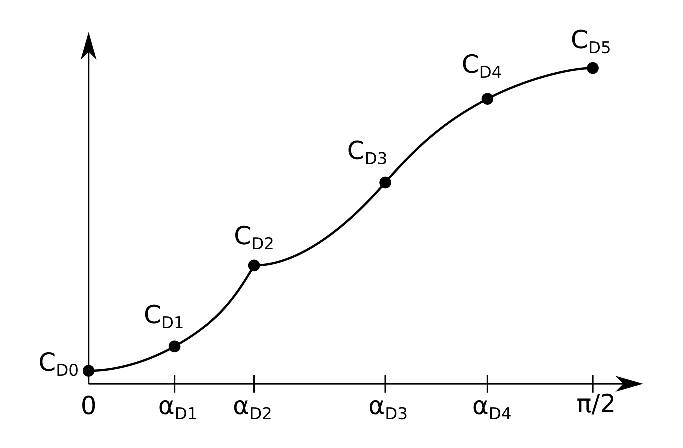
\includegraphics[width=120mm]{eps/approx_cx.eps}
  \caption{Drag coefficient approximation}
\end{figure}

Drag coefficient is given by the following expressions:
\begin{multline}
  C_D =
  \frac{
    \left( \alpha^2 - \alpha_{D2}^2 \right)
    \left( \alpha^2 - \alpha_{D1}^2 \right)
  }
  {
    \alpha_{D1}^2 \alpha_{D2}^2
  } C_{D0}
  +
  \frac{
    \left( \alpha^2 - \alpha_{D2}^2 \right) \alpha^2
  }
  {
    \left( \alpha_{D1}^2 - \alpha_{D2}^2 \right) \alpha_{D1}^2
  } C_{D1}
  +
  \frac{
    \left( \alpha^2 - \alpha_{D1}^2 \right) \alpha^2
  }
  {
    \left( \alpha_{D2}^2 - \alpha_{D1}^2 \right) \alpha_{D2}^2
  } C_{D2} \\
  \mathrm{~for~} -\alpha_{D2} \leq \alpha \leq \alpha_{D2}
\end{multline}
\begin{multline}
  C_D =
  \frac{
    \left( \alpha - \alpha_{D3} \right)
    \left( \alpha - \alpha_{D4} \right)
    \left( \alpha - \frac{\pi}{2} \right)
  }
  {
    \left( \alpha_{D2} - \alpha_{D3} \right)
    \left( \alpha_{D2} - \alpha_{D4} \right)
    \left( \alpha_{D2} - \frac{\pi}{2} \right)
  } C_{D2}
  \\
  +
  \frac{
    \left( \alpha - \alpha_{D2} \right)
    \left( \alpha - \alpha_{D4} \right)
    \left( \alpha - \frac{\pi}{2} \right)
  }
  {
    \left( \alpha_{D3} - \alpha_{D2} \right)
    \left( \alpha_{D3} - \alpha_{D4} \right)
    \left( \alpha_{D3} - \frac{\pi}{2} \right)
  } C_{D3}
  +
  \frac{
    \left( \alpha - \alpha_{D2} \right)
    \left( \alpha - \alpha_{D3} \right)
    \left( \alpha - \frac{\pi}{2} \right)
  }
  {
    \left( \alpha_{D4} - \alpha_{D2} \right)
    \left( \alpha_{D4} - \alpha_{D3} \right)
    \left( \alpha_{D4} - \frac{\pi}{2} \right)
  } C_{D4}
  \\
  +
  \frac{
    \left( \alpha - \alpha_{D2} \right)
    \left( \alpha - \alpha_{D3} \right)
    \left( \alpha - \alpha_{D4} \right)
  }
  {
    \left( \frac{\pi}{2} - \alpha_{D2} \right)
    \left( \frac{\pi}{2} - \alpha_{D3} \right)
    \left( \frac{\pi}{2} - \alpha_{D4} \right)
  } C_{D5}
  \\
  \mathrm{~for~} -\frac{\pi}{2} \leq \alpha < -\alpha_{D2}
  \mathrm{~and~} \alpha_{D2} < \alpha \leq \frac{\pi}{2}
\end{multline}

Data available in \cite{NACA-TN-3361} and \cite{SheldahiKlimas1981} can be used to approximate aerodynamic characteristics outside linear range of the lift.

\section{Finite Wing Aerodynamic Characteristics}

Aerodynamic characteristics of the finite wing can be estimated within linear range of the lift.

Lift curve slope is given as follows: \cite{Corke2003}
\begin{equation}
  \frac{dC_L}{d\alpha}
  =
  \frac{
    2\pi A
  }
  {
    2
    +
    \sqrt{ 4 + A^2 \left( 1 + \tan^2 \Lambda_{t/c} \right) }
  }
\end{equation}

The finite wing lift coefficient within linear range is given by the following formula: \cite{Corke2003}
\begin{equation}
  C_L = C_{L \alpha = 0} + \frac{dC_L}{d \alpha} \alpha
\end{equation}

The finite wing maximum lift coefficient is given by: \cite{Raymer1992}
\begin{equation}
  C_{L,max} = 0.9 C_{L,max \infty} \cos \Lambda_{t/c}
\end{equation}

The finite wing drag coefficient is given as follows. \cite{Corke2003}
\begin{equation}
  C_D = C_{D0} + \frac{C_L^2}{\pi A e}
\end{equation}

\section{Horizontal Tail Incidence}

Equilibrium of moments acting on an aircraft is given by the following equation:
\begin{equation}
  \label{eq-aero-equilibrium-moments}
  r_{CG} mg + \frac{1}{2} \rho V^2 S \hat c C_m
  =
  l_h \frac{1}{2} \rho V^2 S_h C_{L,h}
\end{equation}

Horizontal stabilizer lift coefficient is given as follows:
\begin{equation}
  \label{eq-aero-lift-coef-stab-h}
  C_{L,h}
  =
  \left(
    \alpha + i_h - \alpha \frac{\partial \epsilon}{\partial \alpha}
  \right)
  \frac{d C_{L,h}}{d \alpha}
\end{equation}

Where downwash derivative is given as: \cite{Paturski09}
\begin{equation}
  \frac{\partial \epsilon}{\partial \alpha}
  =
  \frac{2a}{\pi A}
\end{equation}

Substituting equation (\ref{eq-aero-lift-coef-stab-h}) into (\ref{eq-aero-equilibrium-moments}) gives:
\begin{equation}
  r_{CG} mg + \frac{1}{2} \rho V^2 S \hat c C_m
  =
  l_h \frac{1}{2} \rho V^2 S_h
  \left(
  \alpha + i_h - \alpha \frac{\partial \epsilon}{\partial \alpha}
  \right)
  \frac{d C_{L,h}}{d \alpha}
\end{equation}

Solving this equation for horizontal tail incidence angle gives:
\begin{equation}
  \label{eq-aero-incidence-angle}
  i_h = 
  \frac{ 2 r_{CG} mg + \rho V^2 S \hat c C_m }
  { l_h \rho V^2 S_h \cfrac{d C_{L,h}}{d \alpha} }
  -
  \alpha \left( 1 - \frac{\partial \epsilon}{\partial \alpha} \right)
\end{equation}

Equilibrium of forces acting on an aircraft in level flight is given by the following equation:
\begin{equation}
  \label{eq-aero-equilibrium-forces}
  mg = \frac{1}{2} \rho V^2 S C_L
\end{equation}

Aircraft lift coefficient is given as follows:
\begin{equation}
  \label{eq-aero-lift-coef}
  C_L = C_{L0} + \alpha \frac{d C_L}{d \alpha}
\end{equation}

Substituting equation (\ref{eq-aero-lift-coef}) into (\ref{eq-aero-equilibrium-forces}) gives:
\begin{equation}
  mg = \frac{1}{2} \rho V^2 S
  \left( C_{L0} + \alpha \frac{d C_L}{d \alpha} \right)
\end{equation}

Solving this equation for angle of attack gives:
\begin{equation}
  \label{eq-aero-angle-of-attack}
  \alpha = 
  \frac{ 2mg - \rho V^2 S C_{L0} }{ \rho V^2 S \cfrac{d C_L}{d \alpha} }
\end{equation}

Substituting equation (\ref{eq-aero-angle-of-attack}) into (\ref{eq-aero-incidence-angle}) gives:
\begin{equation}
  i_h =
  \frac{ 2 r_{CG} mg + \rho V^2 S \hat c C_m }
  { l_h \rho V^2 S_h \cfrac{d C_{L,h}}{d \alpha} }
  -
  \frac{ 2mg - \rho V^2 S C_{L0} }
  { \rho V^2 S \cfrac{d C_L}{d \alpha} }
  \left( 1 - \frac{\partial \epsilon}{\partial \alpha} \right)
\end{equation}

\section{Critical Angle of Attack}

Equilibrium of forces acting on an aircraft in level flight is given by the following equation:
\begin{equation}
  mg = \frac{1}{2} \rho V^2 \left( S C_L + S_h C_{L,h} \right)
\end{equation}

As conventional configuration airplanes have horizontal stabilizer negative incidence angle, it is assumed that horizontal stabilizer is within its lift linear range when maximum lift coefficient is reached.
\begin{equation}
  mg = \frac{1}{2} \rho V^2
  \left[
    S C_L
    +
    S_h \left(
      \alpha_{cr} + i_h
      -
      \alpha_{cr} \frac{\partial \epsilon}{\partial \alpha}
    \right)
    \frac{d C_{L,h}}{d \alpha}
  \right]
\end{equation}

Solving this equation for the maximum lift coefficient gives:
\begin{equation}
  \label{eq-aero-lift-coef-max-1}
  C_{L,max} = 
  \frac{
    mg - \cfrac{1}{2} \rho V_{stall}^2 S_h
    \left(
      \alpha_{cr} + i_h
      -
      \alpha_{cr} \cfrac{\partial \epsilon}{\partial \alpha}
    \right)
    \cfrac{d C_{L,h}}{d \alpha}
  }
  {
    \cfrac{1}{2} \rho V_{stall}^2 S
  }
\end{equation}

Assuming that maximum lift coefficient is within linear range:
\begin{equation}
  \label{eq-aero-lift-coef-max-2}
  C_{L,max} =  C_{L0} + \alpha_{cr} \frac{d C_L}{d \alpha}
\end{equation}

Substituting equation (\ref{eq-aero-lift-coef-max-2}) into (\ref{eq-aero-lift-coef-max-1}) gives:
\begin{equation}
  C_{L0} + \alpha_{cr} \frac{d C_L}{d \alpha} =
  \frac{
    mg - \cfrac{1}{2} \rho V_{stall}^2 S_h
    \left(
      \alpha_{cr} + i_h
      -
      \alpha_{cr} \cfrac{\partial \epsilon}{\partial \alpha}
    \right)
    \cfrac{d C_{L,h}}{d \alpha}
  }
  {
    \cfrac{1}{2} \rho V_{stall}^2 S
  }
\end{equation}

Solving this equation for critical angle of attack gives
\begin{equation}
  \label{eq-aero-alpha-critical}
  \alpha_{cr} =
  \frac{
    2mg - \rho V_{stall}^2
    \left(
      S_h i_h \cfrac{d C_{L,h}}{d \alpha}
      +
      S C_{L0}
    \right)
  }
  {
    \rho V_{stall}^2
    \left[
      S \cfrac{d C_L}{d \alpha}
      +
      S_h \left( 1 - \cfrac{\partial \epsilon}{\partial \alpha} \right)
      \cfrac{d C_{L,h}}{d \alpha}
    \right]
  }
\end{equation}
